\documentclass[handout,mathserif,10pt]{beamer}

\mode<presentation>
{
  \usetheme{shadow}
  \usecolortheme{crane}
  \setbeamercovered{transparent}
  \useoutertheme{infolines}
}

%\usepackage[german]{babel}
%\usepackage[latin1]{inputenc}

\usepackage{times}
\usepackage[T1]{fontenc}
\usepackage{amssymb,amsmath,amsthm, amsbsy, bm}


\title[Term Structure and Credit Spread Estimation with \textsf{R}] % (optional, nur bei langen Titeln n�tig)
{Term Structure and \\Credit Spread Estimation with \textsf{R}}

\author[Robert Ferstl]{Robert Ferstl}

\institute{Institute for Operations Research\\WU Wien\\
\begin{center}
	\includegraphics[width=0.20\textwidth]{euro.jpg}
\end{center}}

\date[Robert Ferstl]
{July 5, 2006}


\pgfdeclareimage[height=1.0cm]{wu-logo}{wu-logo}
\logo{\pgfuseimage{wu-logo}}

\begin{document}

\begin{frame}
  \titlepage
\end{frame}

\begin{frame}
  \frametitle{Basic principles of bond pricing}
  \begin{itemize}
    \item coupon bond which matures in $n$ years
    \item investor gets at the times $i=1,\dots n$ coupon payments $C$ and a redemption payment $R$ at $t=n$
    \item \textcolor{craneblue}{\textbf{clean price}} $p_c$ is quoted on the market
    \item seller also receives \textcolor{craneblue}{\textbf{accrued interest}} for holding the bond over the period since the last coupon payment
  	\begin{equation*}
  \label{accruedinterest}
  a=\frac{\mbox{number of days since last coupon}}{\mbox{number of days in current coupon period}}C
\end{equation*}
	\item investor has to pay the \textcolor{craneblue}{\textbf{dirty price}} $p_d$
\item bond pricing equation with continuous compounding
\begin{equation*}
  \label{bondpriceeq}
  p_c+a = C\sum_{i=1}^ne^{-s_im_i}+Re^{-s_nm_n}
\end{equation*}
\end{itemize}
\end{frame}



\begin{frame}
\frametitle{Basic principles of bond pricing}
  \begin{itemize}
\item \textcolor{craneblue}{\textbf{yield to maturity}}
\begin{equation*}
  \label{yield}
  p_c+a=C\sum_{i=1}^ne^{-ym_i}+Re^{-ym_n}
\end{equation*}
\item  equivalent formulation of the bond price equation uses the \textcolor{craneblue}{\textbf{discount factors}} $d_i=\delta(m_i)=e^{-s_im_i}$
\item continuous \textcolor{craneblue}{\textbf{discount function}} $\delta(\cdot)$ is formed by interpolation of the discount factors
  \begin{equation*}
  \label{bondprceq2}
  p_c+a=C\sum_{i=1}^n\delta(m_i)+\delta(m_n)R 
  \end{equation*}
  \item implied $j$-period \textcolor{craneblue}{\textbf{forward rate}}
  \begin{equation*}
  \label{forwrate}
  f_{t|j}=\frac{js_j-ts_t}{j-t}
\end{equation*}
  \item \textcolor{craneblue}{\textbf{duration}} is a weighted average of time to cash flows
  \begin{equation*}
  \label{duration} D=\frac{1}{p_c+a}\left[C\sum_{i=1}^n\delta(m_i)m_i+\delta(m_n)Rm_n\right]
\end{equation*}
\end{itemize}
\end{frame}

\begin{frame}
  \frametitle{Term structure estimation} 
  \begin{itemize}
  \item estimate zero-coupon yield curves and credit spread curves from market data
  \item usual way for calculation of \textcolor{craneblue}{\textbf{credit spread curves}} 
\begin{equation*}
  \label{spread}
  c_i(m)=s_i(m)-s_{ref}(m)
\end{equation*}
  \item parsimonious approach widely used by central banks
  \end{itemize}
\begin{center}
	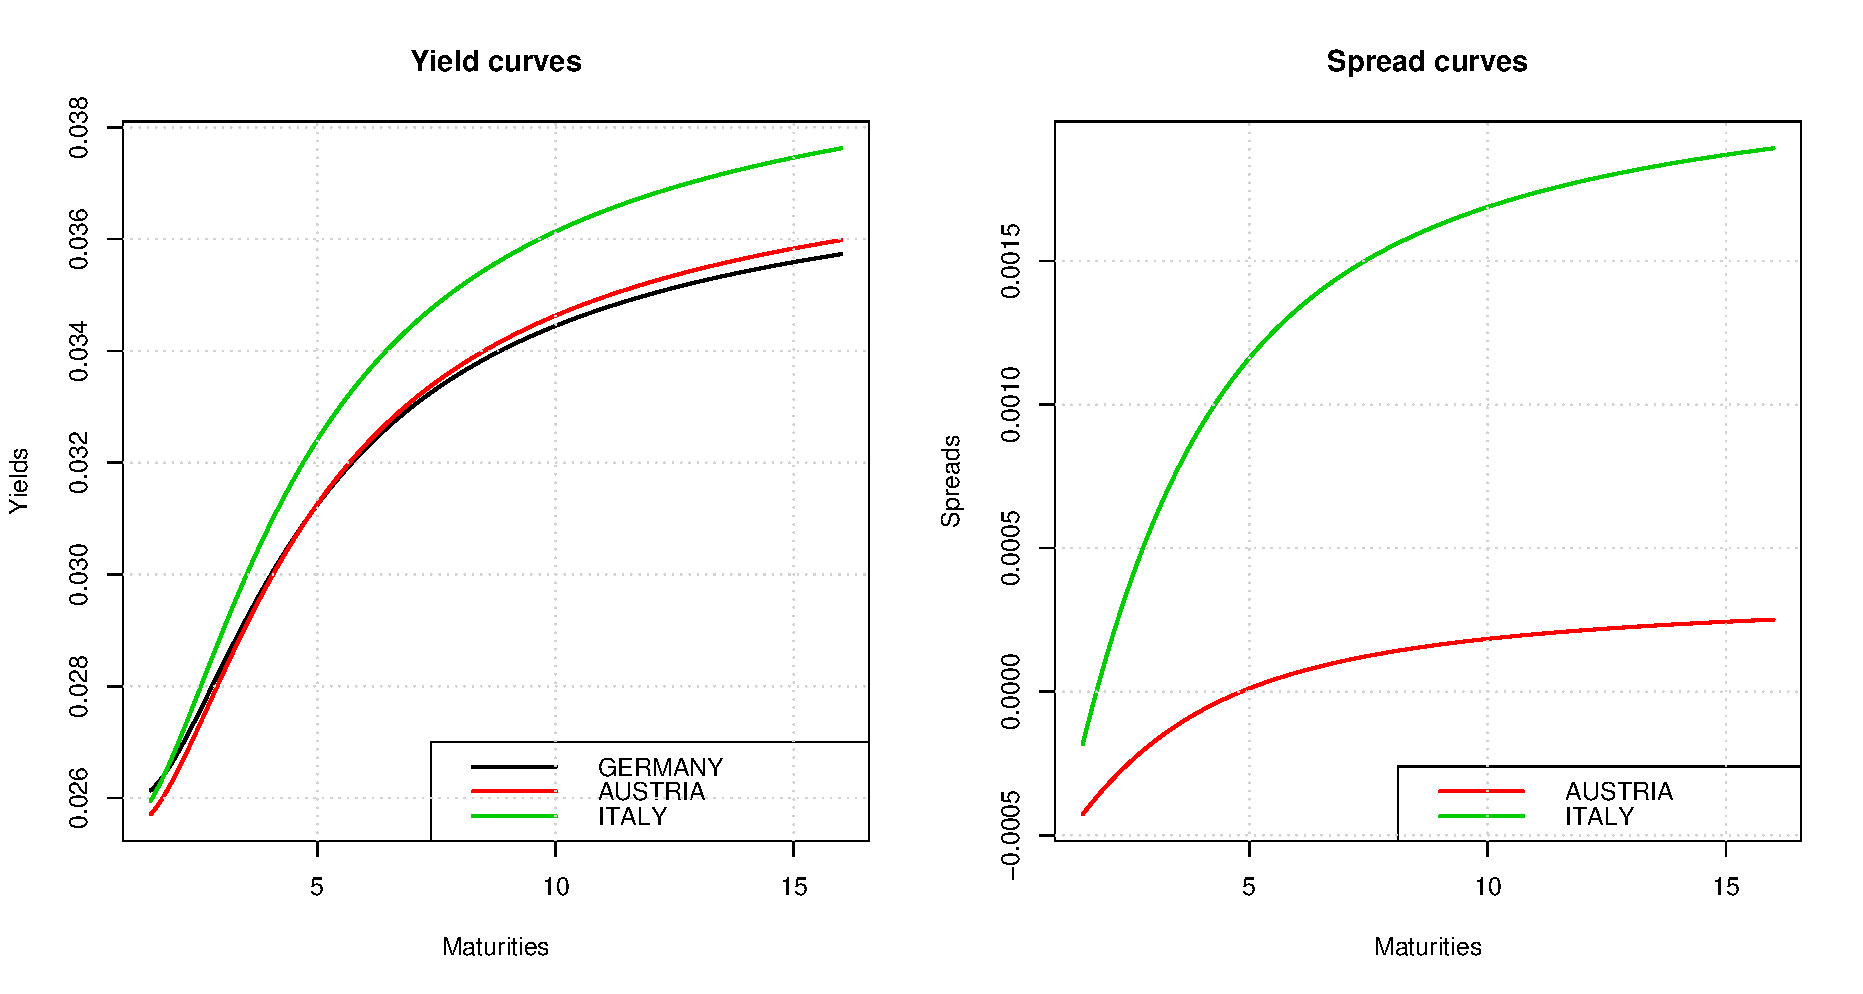
\includegraphics[width=0.97\textwidth]{curves}
\end{center}
\end{frame}

\begin{frame}
  \frametitle{Nelson and Siegel (1987) approach}
  %\framesubtitle{Untertitel sind optional.}
   \begin{beamerboxesrounded}[shadow=true]{Instantaneous forward rates}
\begin{equation*}
	    f(m,\bm{b}) = \beta_0 + \beta_1 \exp(-\frac{m}{\tau_1}) + \beta_2 \frac{m}{\tau_1} \exp(-\frac{m}{\tau_1})
\end{equation*}
 \end{beamerboxesrounded} 
\begin{center}
	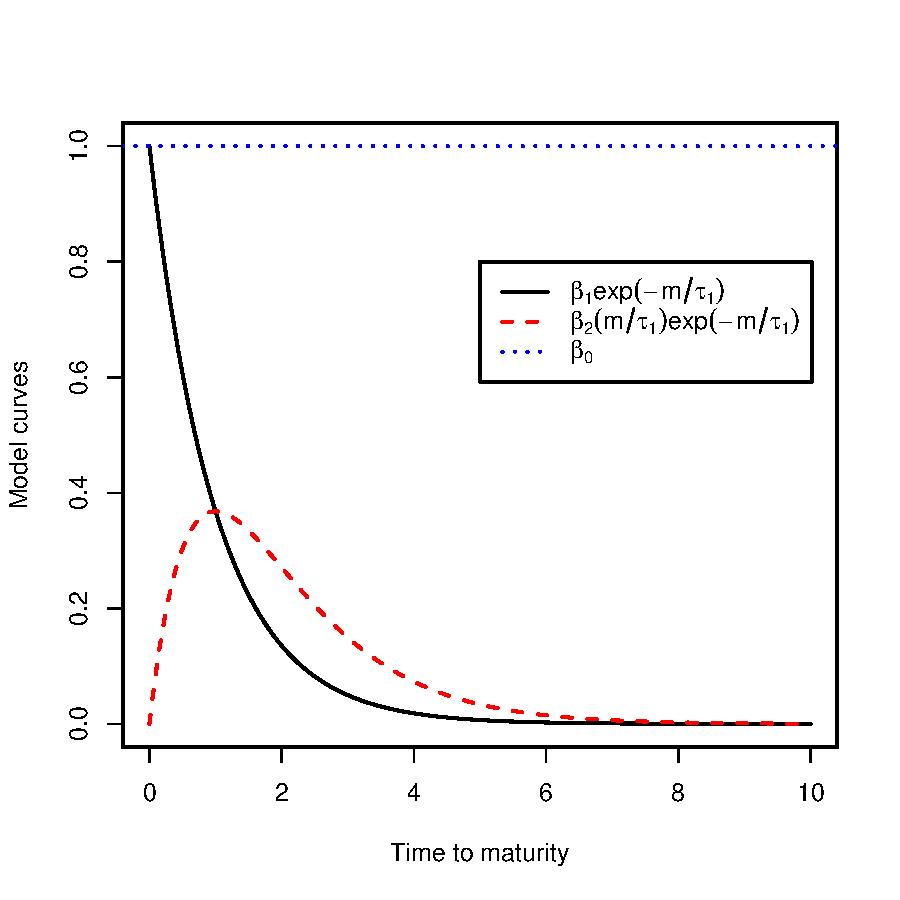
\includegraphics[width=0.65\textwidth]{fignelson}
\end{center}
\end{frame}

\begin{frame}
  \frametitle{Nelson and Siegel (1987) approach}
 \begin{beamerboxesrounded}[shadow=true]{Spot rates}
\begin{equation*}\label{nelson}
    s(m,\bm{b}) = \beta_0 + \beta_1\frac{1-\exp(-\frac{m}{\tau_1})}{\frac{m}{\tau_1}} + \beta_2\left(\frac{1-\exp(-\frac{m}{\tau_1})}{\frac{m}{\tau_1}} - \exp(-\frac{m}{\tau_1})\right)
\end{equation*}
\end{beamerboxesrounded}
\vspace{0.5cm}
\begin{beamerboxesrounded}[shadow=true]{Objective function}
\begin{equation*}
    \bm{b}_{opt} = \min_{\bm{b}}\sum^{n}_{i=1}\omega_i\left(\hat{P}_i-P_i\right)^{2}\quad\quad\mbox{weighted price errors}
\end{equation*} 
\begin{equation*}
    \bm{b}_{opt} = \min_{\bm{b}}\sum^{n}_{i=1}\left(\hat{y}_i-y_i\right)^{2}\quad\quad\mbox{yield errors}
\end{equation*} 
\end{beamerboxesrounded}
\end{frame}

\begin{frame}
  \frametitle{Extensions}
 \begin{itemize}
   \item Svensson (1994) extended the functional form by two additional parameters which allows for a second hump-shape
 \end{itemize}

\begin{beamerboxesrounded}[shadow=true]{Instantaneous forward rates}
\begin{equation*}
	    f(m,\bm{b}) = \beta_0 + \beta_1 \exp(-\frac{m}{\tau_1}) + \beta_2 \frac{m}{\tau_1} \exp(-\frac{m}{\tau_1})+\beta_3 \frac{m}{\tau_2} \exp(-\frac{m}{\tau_2})
\end{equation*}
\end{beamerboxesrounded}

\begin{itemize}
	\item simple calculation method of credit spread curves could lead to twisting curves
	\item Jankowitsch and Pichler (2004) proposed a \textcolor{craneblue}{\textbf{joint estimation method}}, which leads to smoother and more realistic credit spread curves
\end{itemize}

\end{frame}

\begin{frame}
  \frametitle{Multi-curve approach}
  \framesubtitle{Jankowitsch and Pichler (2004)}

\begin{beamerboxesrounded}[shadow=true]{credit spread curve for the $i$-th country}
\begin{equation*}
  \label{multisv}
  c_i(m)= \gamma_{0,i} + \gamma_{1,i}\frac{1-\exp\left(-\frac{m}{\kappa_1}\right)}{\frac{m}{\kappa_1}} + \gamma_{2,i}\exp\left(-\frac{m}{\kappa_1}\right)
\end{equation*}
with parameters $\bm{\kappa}=(\gamma_{0,i},\gamma_{1,i},\gamma_{2,i},\kappa_i)$
\end{beamerboxesrounded}
\vspace{0.5cm}
\begin{beamerboxesrounded}[shadow=true]{zero-coupon yield curve for the $i$-th country}
  \begin{equation*}
  \label{multsv}
  s_i(m)=s_{ref}(m)+c_i(m)
\end{equation*}
\end{beamerboxesrounded}
\vspace{0.5cm}
% \begin{beamerboxesrounded}[shadow=true]{parameters for joint estimation}
%   \begin{equation*}
%     \bm{\alpha}=(\beta_0,\beta_1,\beta_2,\tau_1,;\gamma_{0,1},\gamma_{1,1},\gamma_{2,1},\kappa_1;\dots;\gamma_{0,C},\gamma_{1,C},\gamma_{2,C},\kappa_C)
%   \end{equation*}
% \end{beamerboxesrounded}

\begin{itemize}
\item parameters for joint estimation:\\ \vspace{0.2cm}
 $\bm{\alpha}=(\beta_0,\beta_1,\beta_2,\tau_1,;\gamma_{0,1},\gamma_{1,1},\gamma_{2,1},\kappa_1;\dots;\gamma_{0,C},\gamma_{1,C},\gamma_{2,C},\kappa_C)$
\end{itemize}

\end{frame}



\begin{frame}
  \frametitle{Example: Government Bonds I}
  \framesubtitle{Single-curve estimation}
\begin{center}
	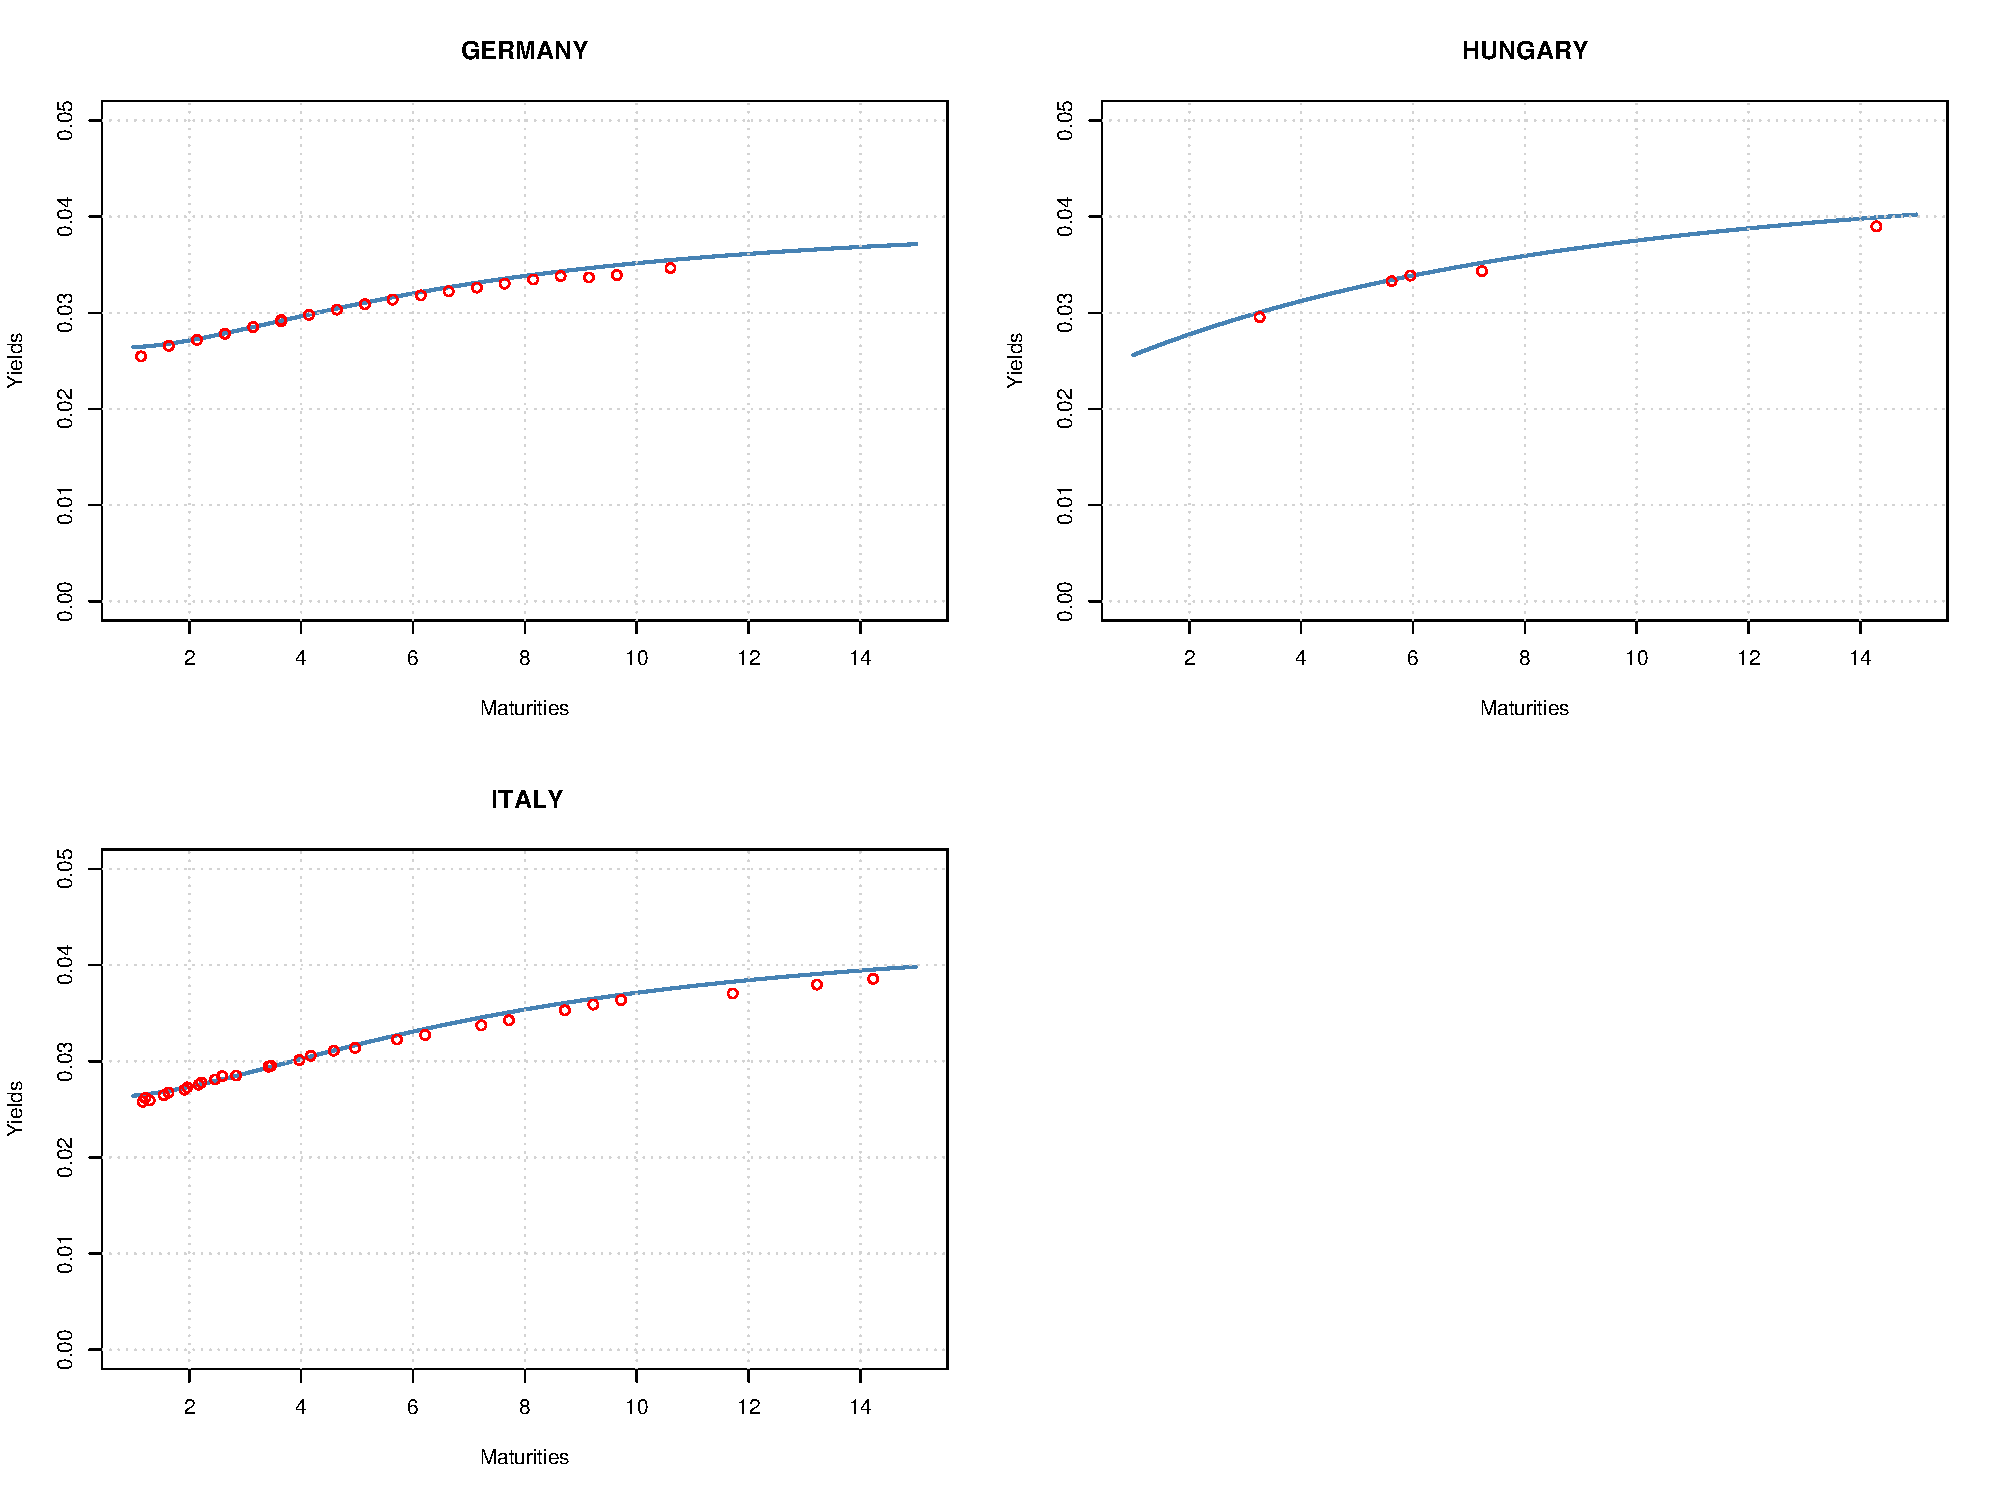
\includegraphics[width=0.97\textwidth]{eurosinglecurveyc}
\end{center}
\end{frame}

\begin{frame}
  \frametitle{Example: Government Bonds II}
\framesubtitle{Single-curve estimation}
\begin{center}
	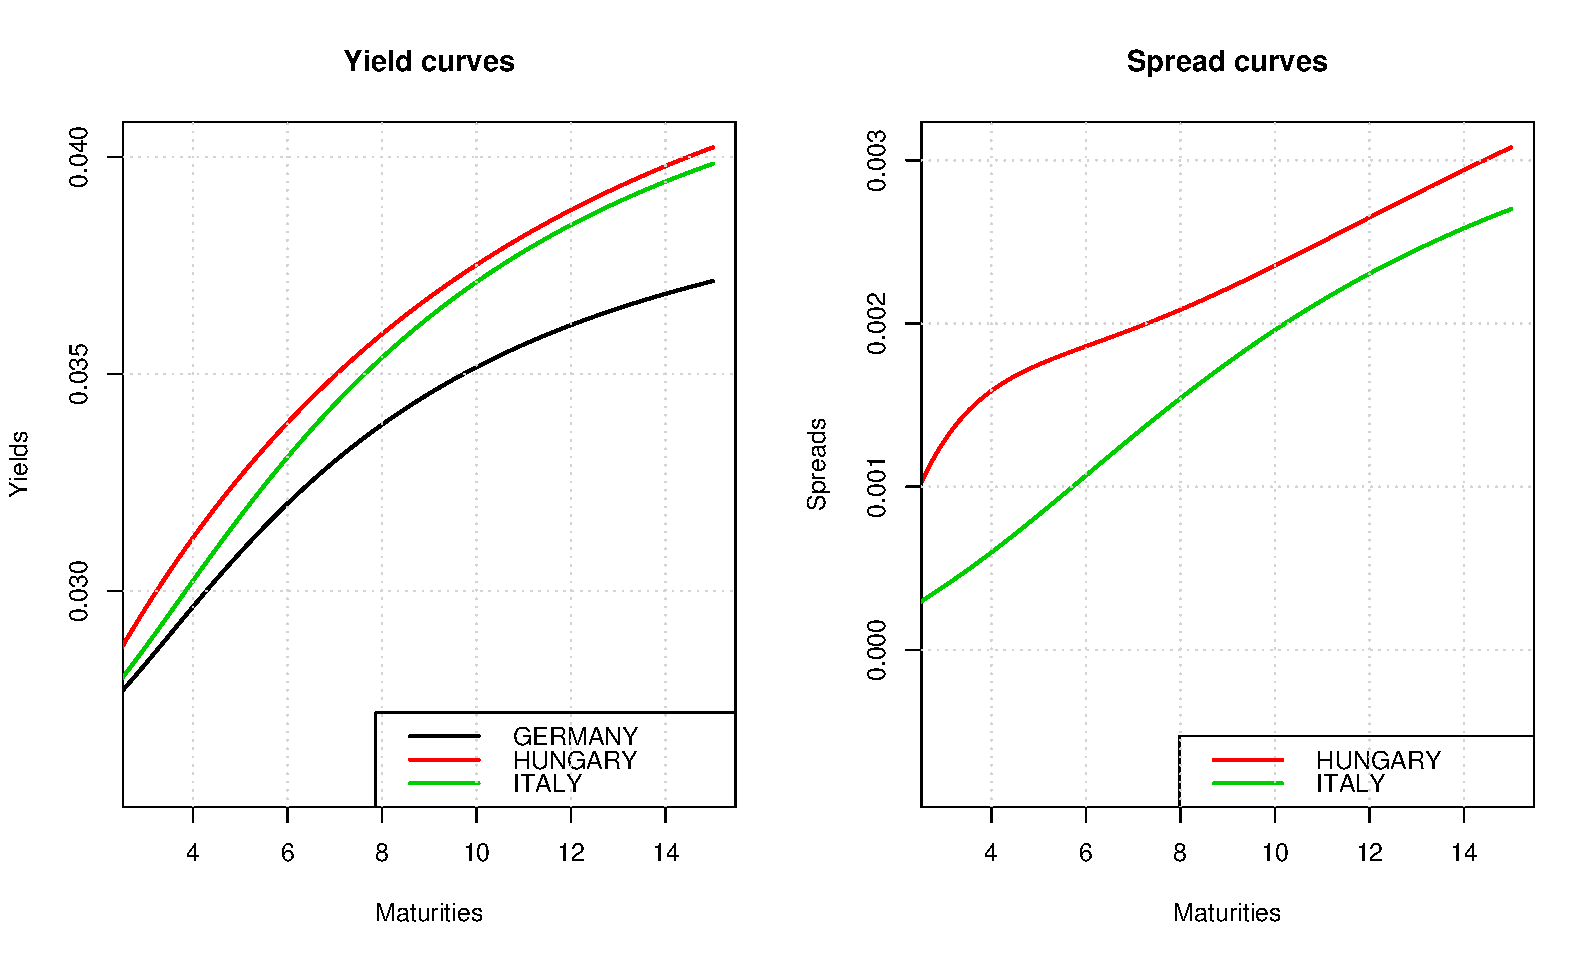
\includegraphics[width=0.97\textwidth]{eurosinglecurve}
\end{center}
\end{frame}

\begin{frame}
  \frametitle{Example: Government Bonds III}
\framesubtitle{Multi-curve estimation}
\begin{center}
	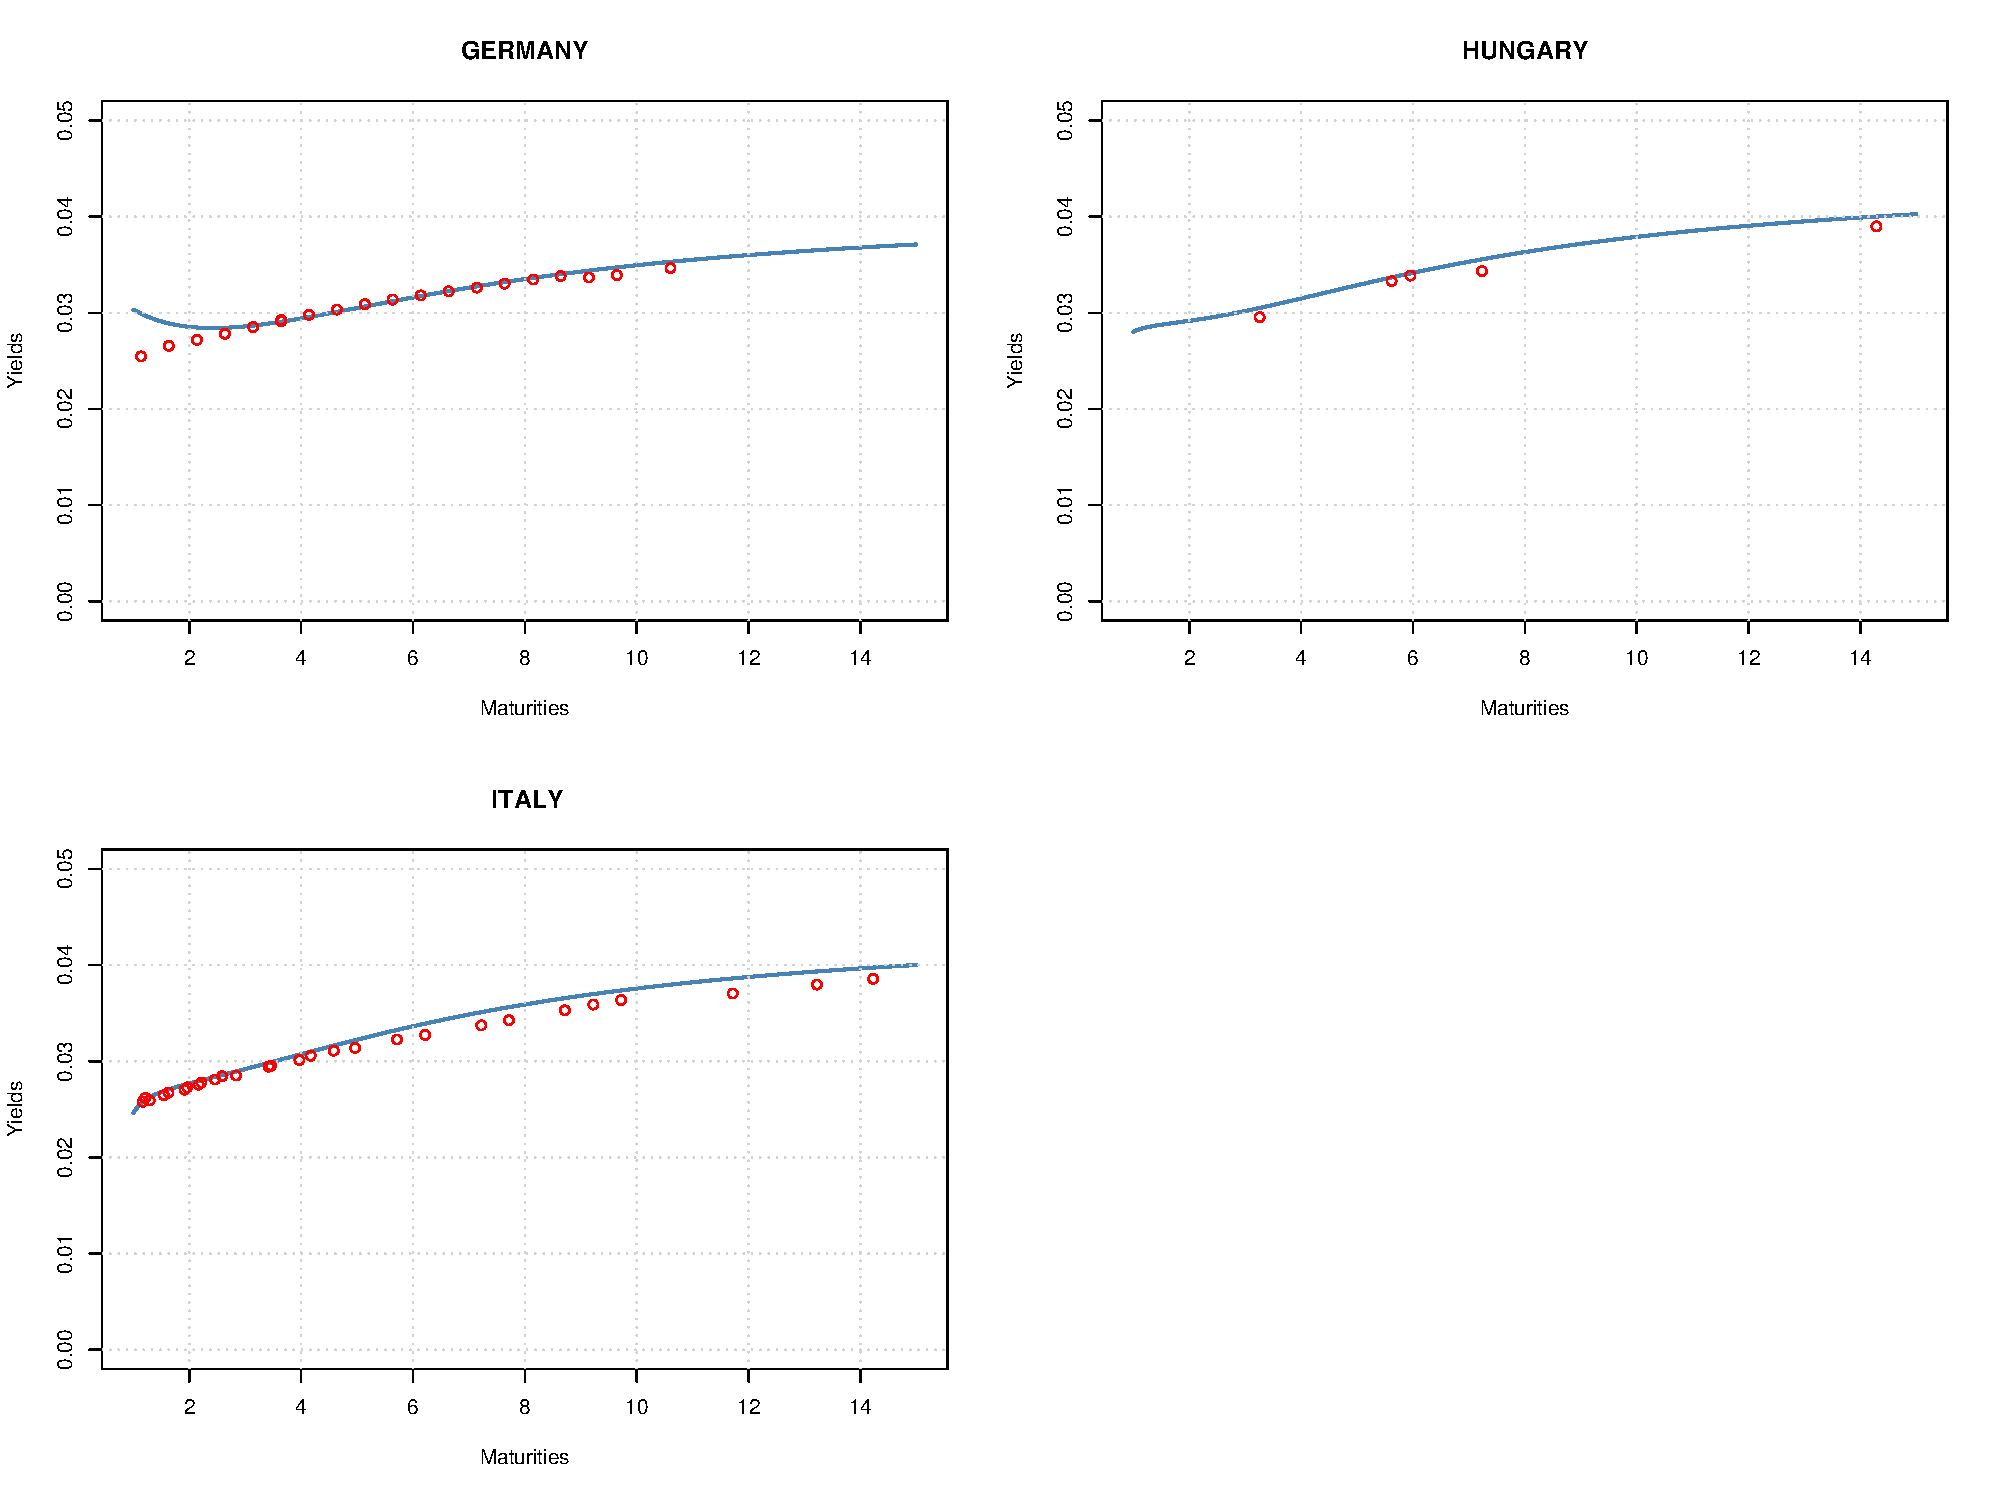
\includegraphics[width=1.00\textwidth]{euromulticurveyc}
\end{center}
\end{frame}

\begin{frame}
  \frametitle{Example: Government Bonds IV}
\framesubtitle{Multi-curve estimation}
\begin{center}
	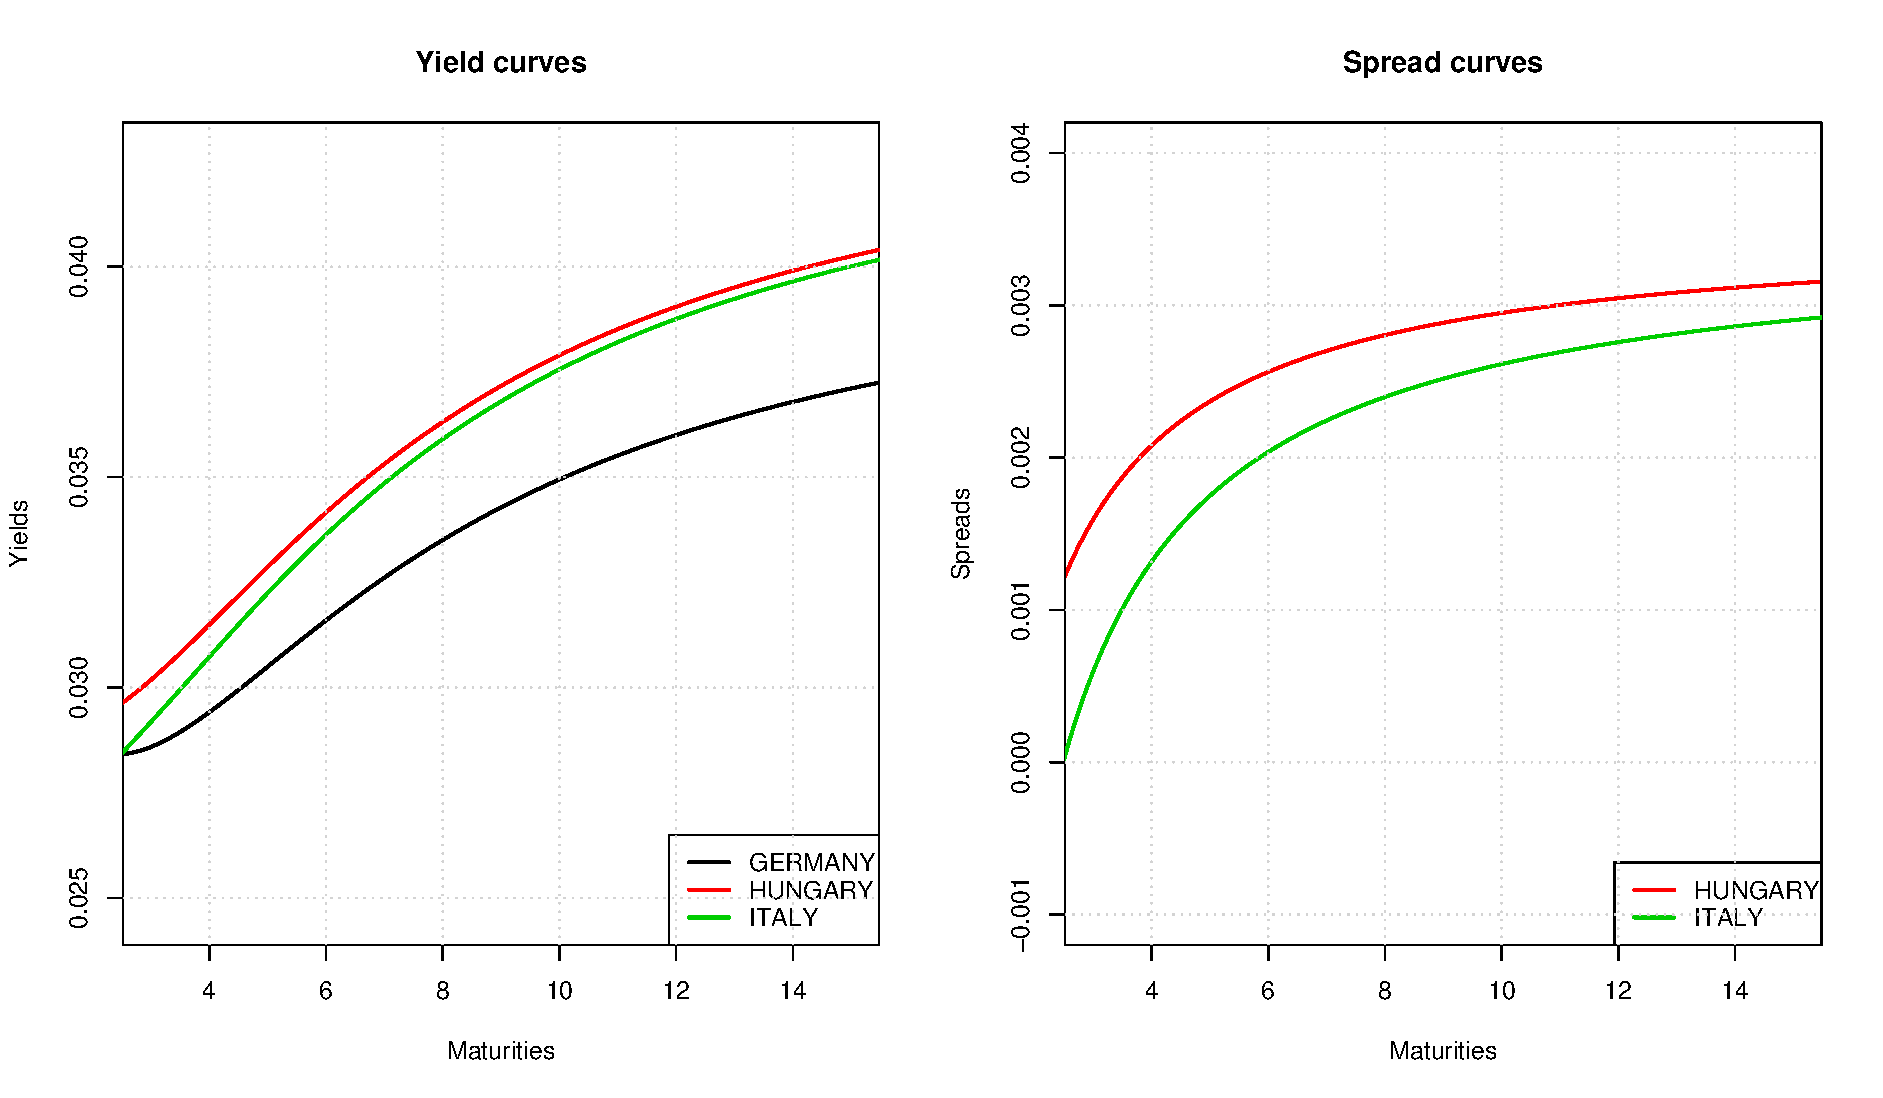
\includegraphics[width=1.00\textwidth]{euromulticurve}
\end{center}
\end{frame}


\begin{frame}
  \frametitle{Example: Corporate Bonds I}
  \framesubtitle{Single-curve estimation}
\begin{center}
	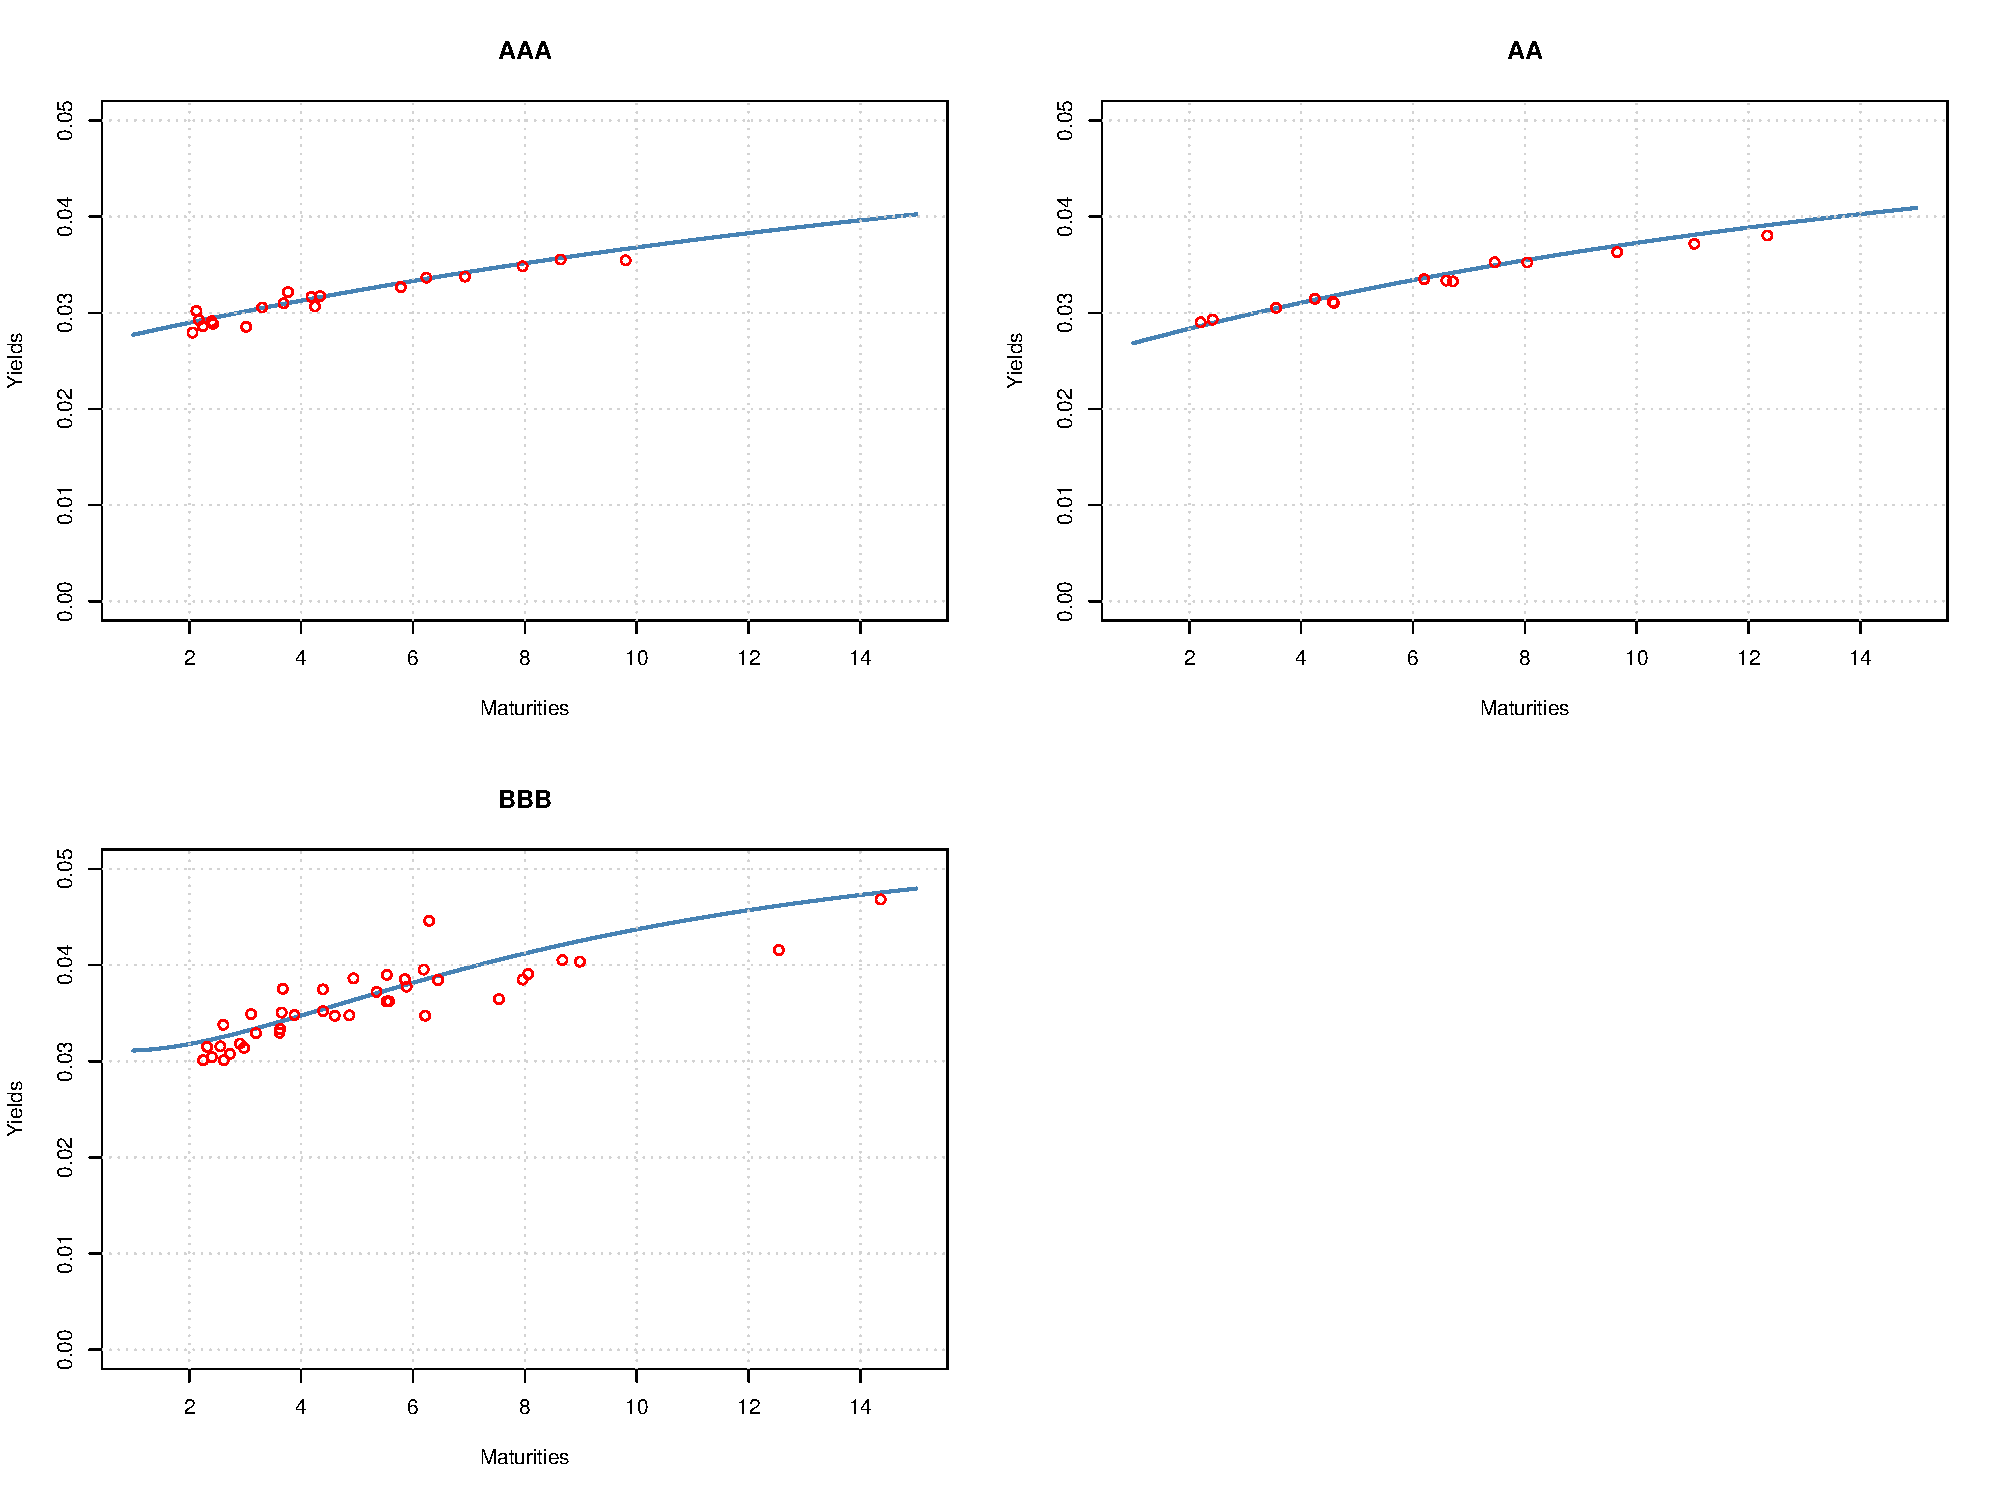
\includegraphics[width=0.97\textwidth]{corpsinglecurveyc}
\end{center}
\end{frame}

\begin{frame}
  \frametitle{Example: Corporate Bonds II}
\framesubtitle{Single-curve estimation}
\begin{center}
	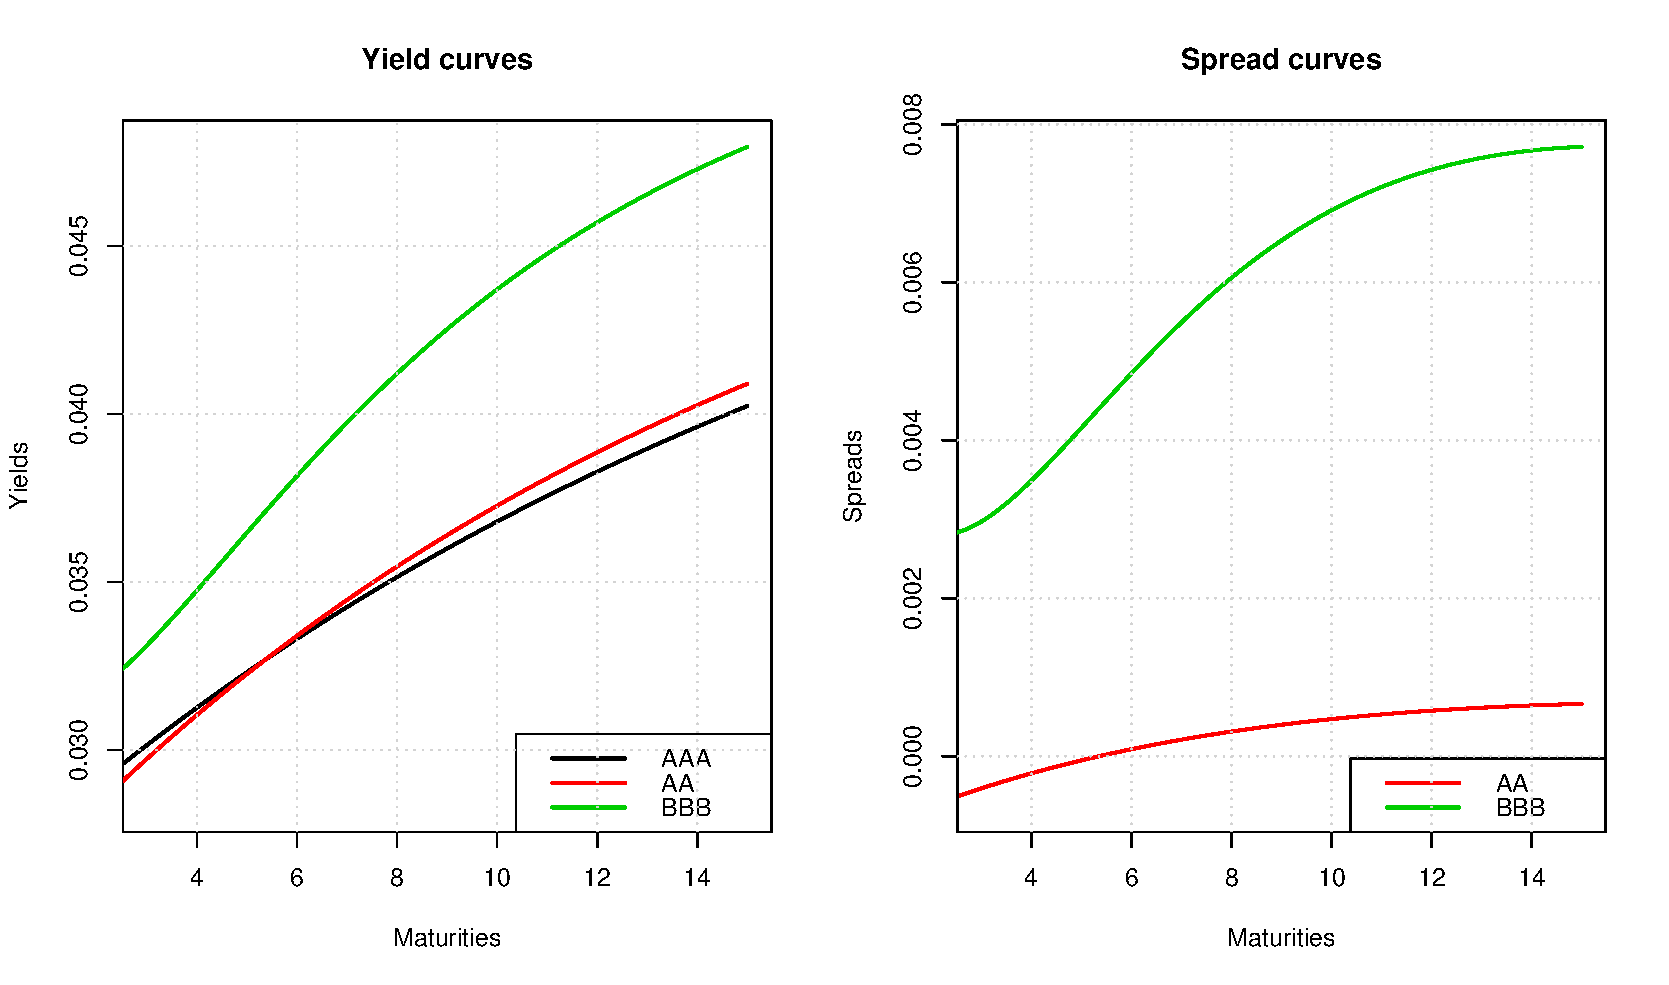
\includegraphics[width=0.97\textwidth]{corpsinglecurve}
\end{center}
\end{frame}

\begin{frame}
  \frametitle{Example: Corporate Bonds III}
\framesubtitle{Multi-curve estimation}
\begin{center}
	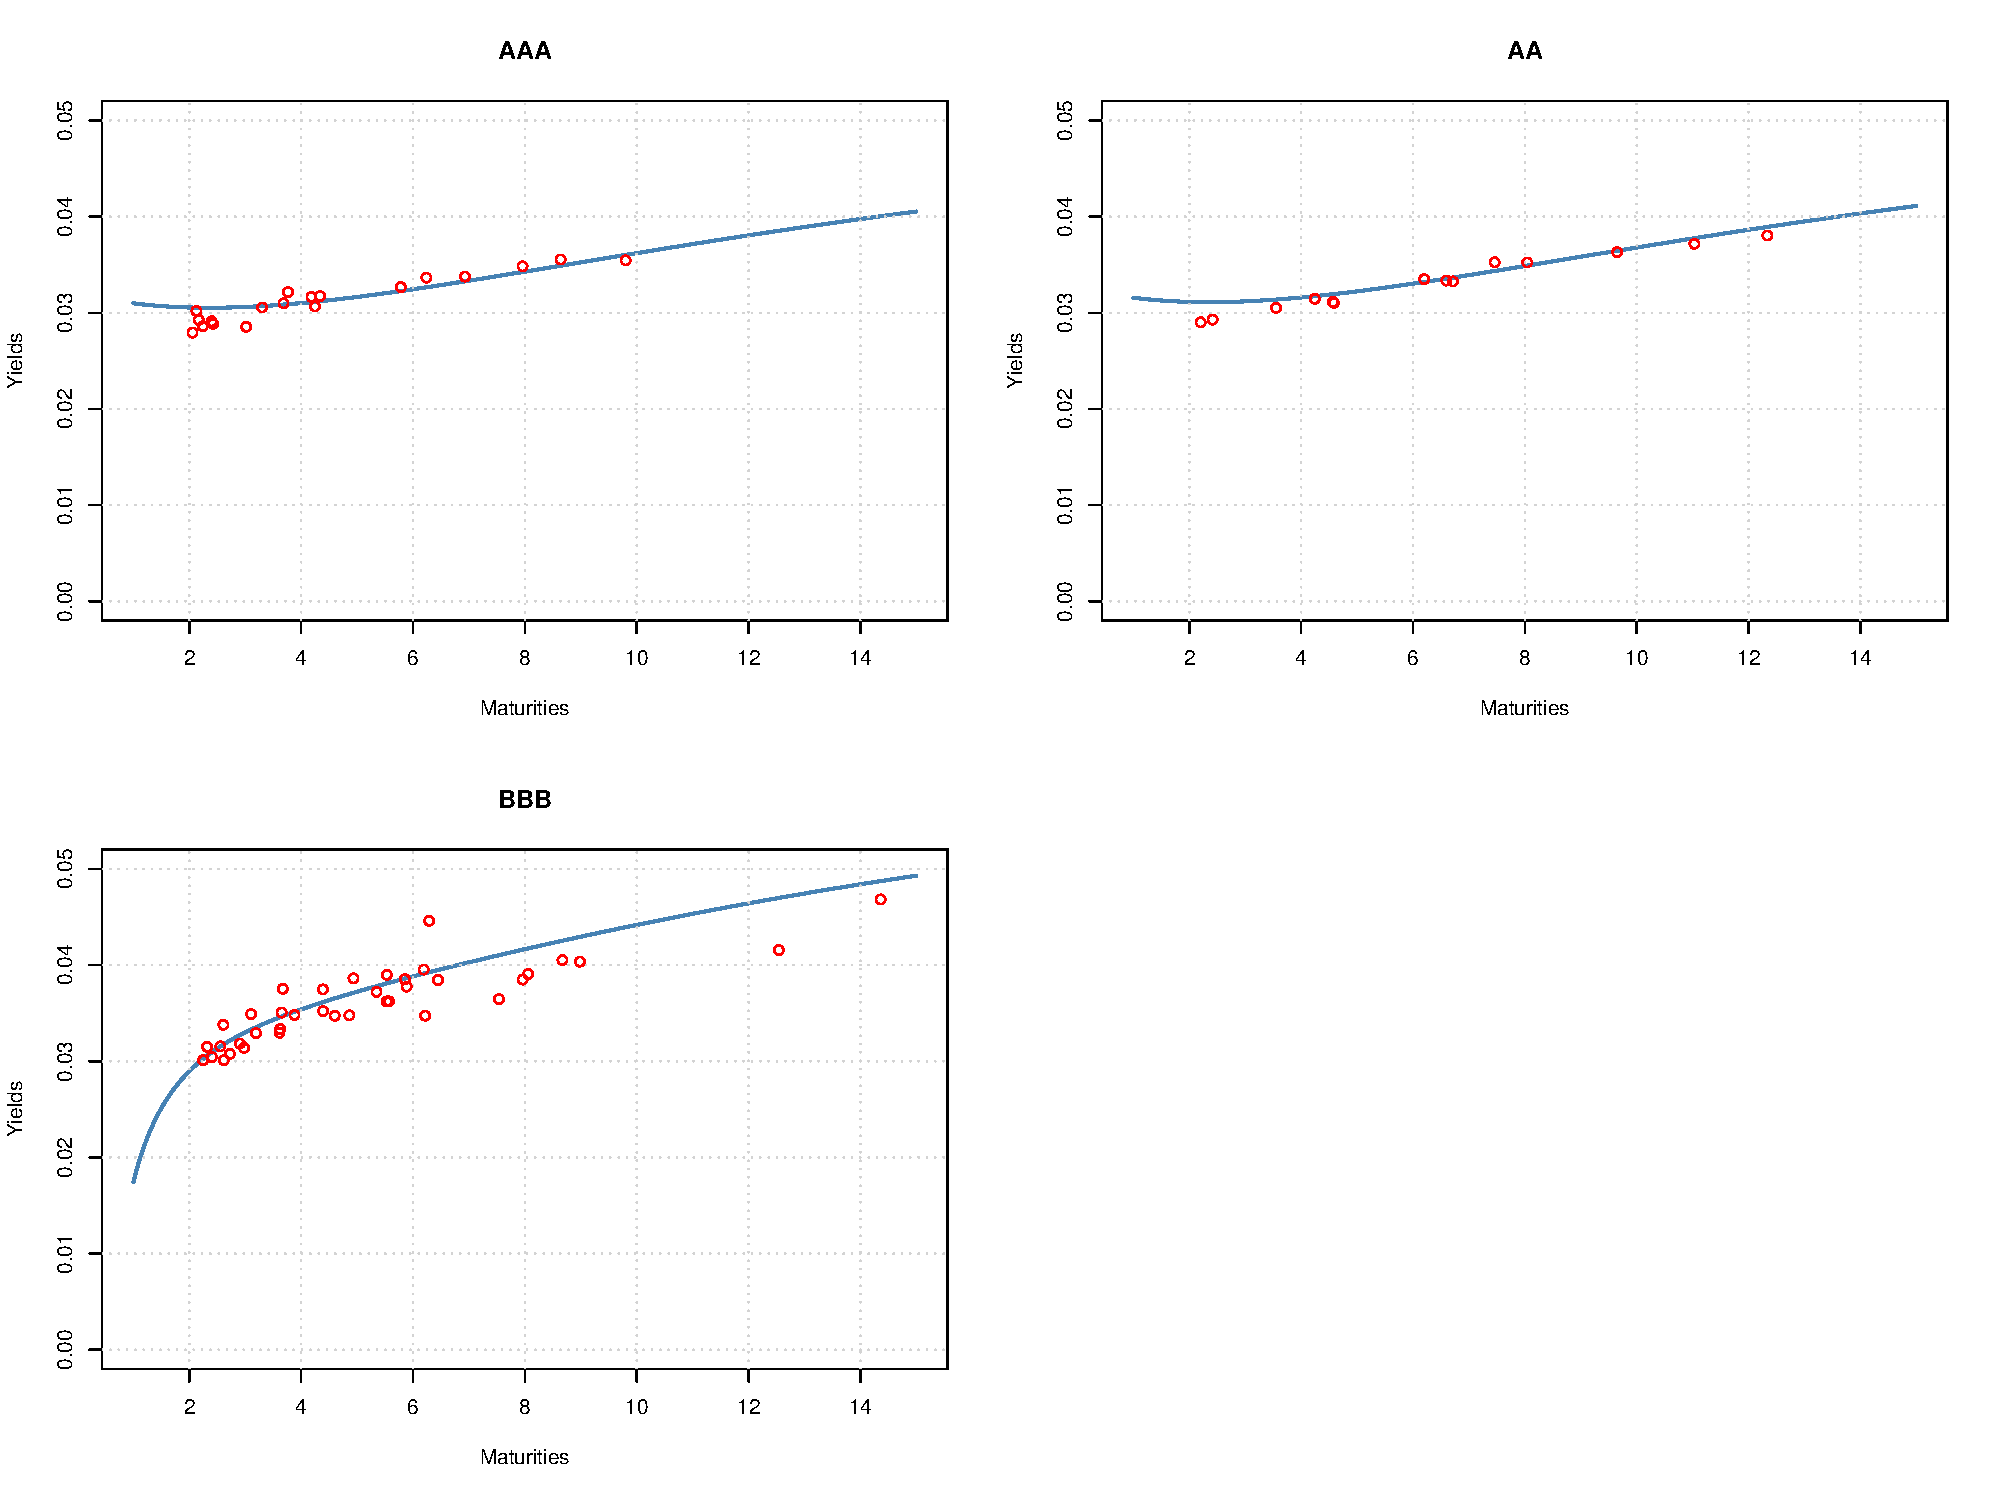
\includegraphics[width=1.00\textwidth]{corpmulticurveyc}
\end{center}
\end{frame}

\begin{frame}
  \frametitle{Example: Corporate Bonds IV}
\framesubtitle{Multi-curve estimation}
\begin{center}
	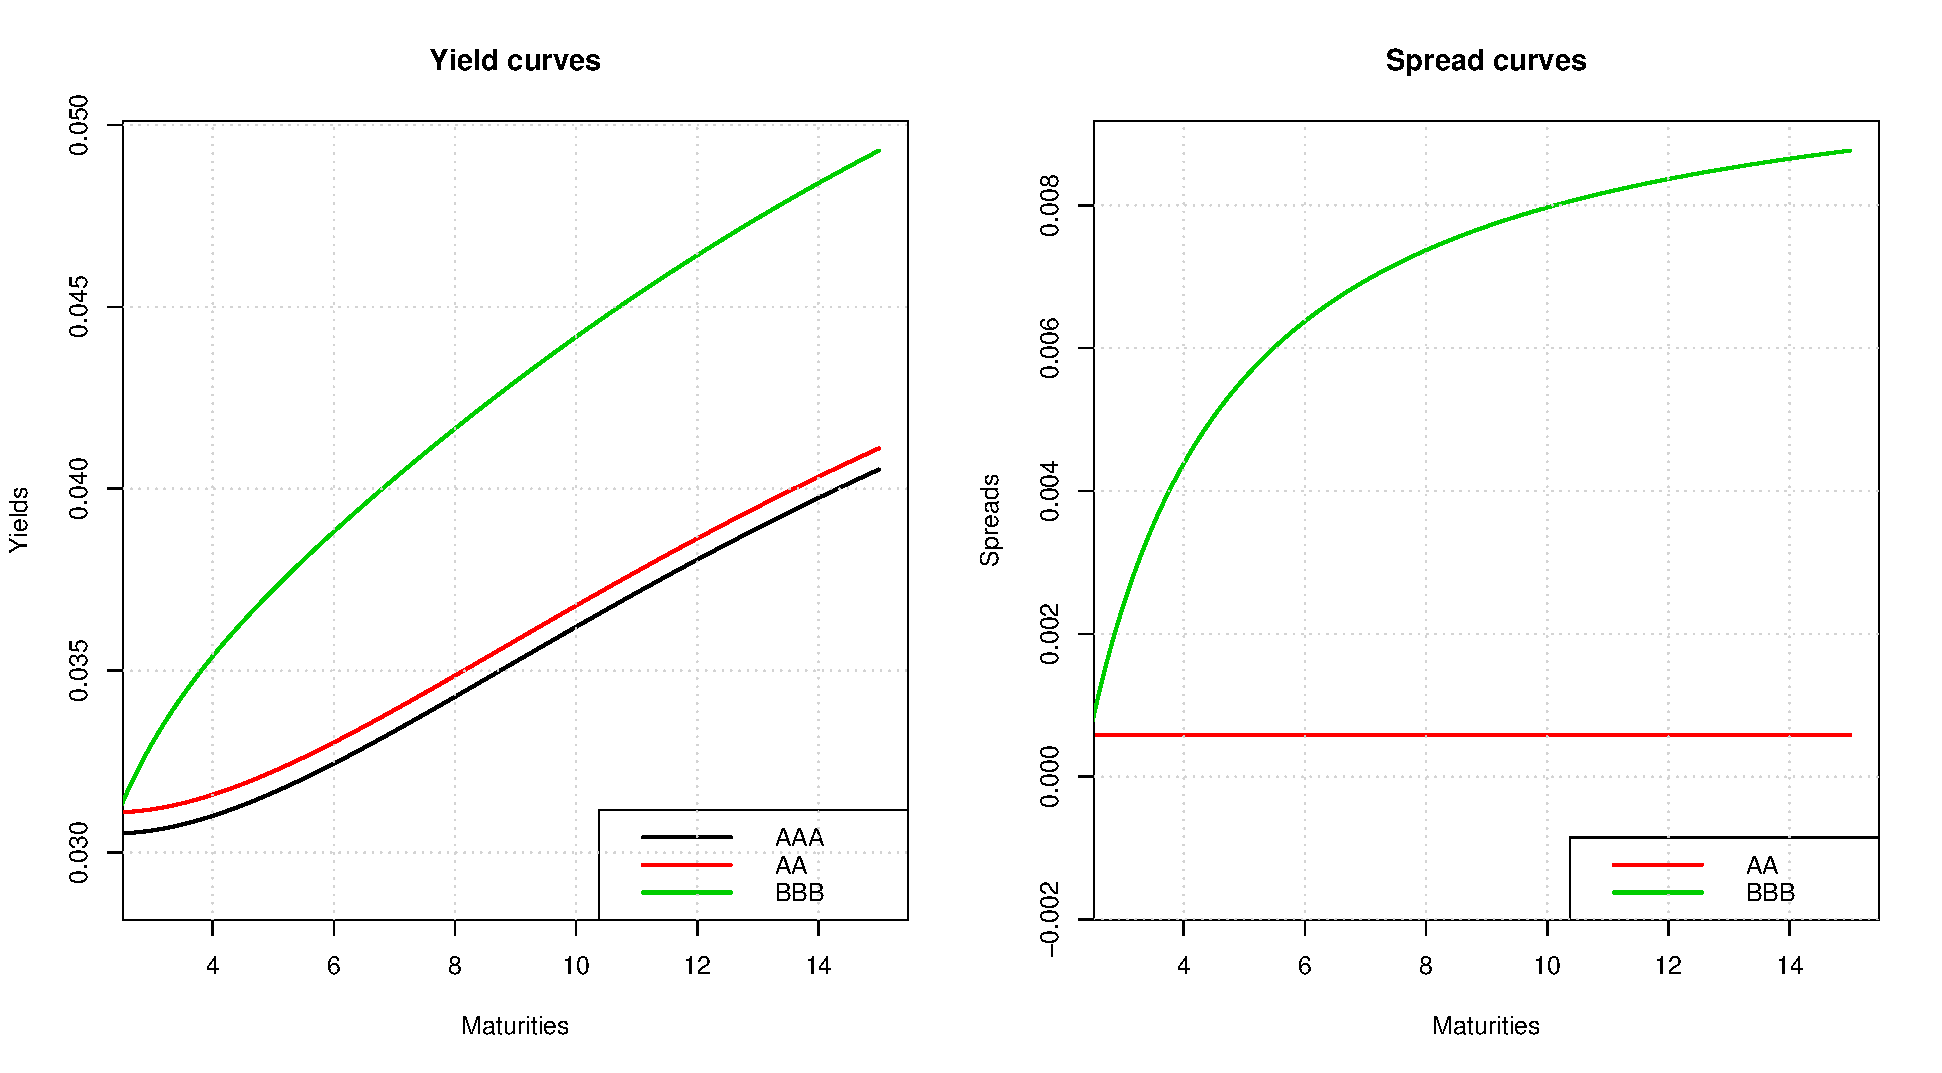
\includegraphics[width=1.00\textwidth]{corpmulticurve}
\end{center}
\end{frame}

\begin{frame}[allowframebreaks]
  \frametitle<presentation>{References}

  \begin{thebibliography}{10}

  \beamertemplatearticlebibitems
  
   \bibitem{BIS2005}
   Bank for International Settlements
   \newblock Zero-coupon yield curves: technical documentation
   \newblock {\em BIS Papers}, No. 25, October 2005
  
  \bibitem{Bolder1999}
   David Bolder, David Streliski
   \newblock Yield Curve Modelling at the Bank of Canada
   \newblock {\em Bank of Canada, Technical Report}, No. 84, 1999
  
    \bibitem{Geyer1999}
    Alois Geyer, Richard Mader
    \newblock Estimation of the Term Structure of Interest Rates - A Parametric Approach
    \newblock {\em OeNB, Working Paper}, No. 37, 1999

\framebreak
  \bibitem{Jankowitsch2004}
    Rainer Jankowitsch, Stefan Pichler
    \newblock Parsimonious Estimation of Credit Spreads
    \newblock {\em The Journal of Fixed Income}, 14(3):49--63, 2004
    
    \bibitem{Nelson1987}
    Charles R. Nelson, Andrew F. Siegel
    \newblock Parsimonious Modeling of Yield Curves
    \newblock {\em The Journal of Business}, 60(4):473--489, 1987
    
    \bibitem{Svensson1994}
    Lars E.O. Svensson
    \newblock Estimating and Interpreting Forward Interest Rates:\\Sweden 1992 -1994
    \newblock {\em National Bureau of Economic Research, \\Technical Report}, No. 4871, 1994

  \end{thebibliography}
\end{frame}

\end{document}
